\documentclass[a4paper,12pt]{article} % тип документа

%  Русский язык

\usepackage{wrapfig}
\usepackage[T2A]{fontenc}			% кодировка
\usepackage[utf8]{inputenc}			% кодировка исходного текста
\usepackage[english,russian]{babel}	% локализация и переносы

\usepackage{indentfirst} %Красная строка
\usepackage[a4paper,top=1.3cm,bottom=2cm,left=1.5cm,right=1.5cm,marginparwidth=0.75cm]{geometry}
\usepackage[usenames]{color}
\usepackage{colortbl}
\usepackage{float}

\usepackage{graphicx}%картинки
\usepackage{textcomp}%Номер
\usepackage{wrapfig}%обтекание текстом теблиц и картинок
%гиперссылки
\usepackage{hyperref}
\usepackage[rgb]{xcolor}
\hypersetup{     %гипперсылки
 colorlinks=true, %false:ссылки в рамках
 urlcolor=blue   %на URL
 }
% Заметки
\usepackage{todonotes}
% Номера формул(необязятельна, см. по ситуации)
%\mathtoolsset{showonlyrefs=true} % Показывать номера только у тех формул, на которые есть \eqref{} в тексте.

% Математика
\usepackage{amsmath,amsfonts,amssymb,amsthm,mathtools} 
\usepackage{wasysym}

\usepackage{euscript} % Шрифт Евклид
\usepackage{mathrsfs} % Красивый матшрифт

\begin{document}

\begin{titlepage}
\begin{center}
    {\large МОСКОВСКИЙ ФИЗИКО-ТЕХНИЧЕСКИЙ ИНСТИТУТ (НАЦИОНАЛЬНЫЙ ИССЛЕДОВАТЕЛЬСКИЙ УНИВЕРСИТЕТ)}
\end{center}
\begin{center}
    {\largeФизтех-школа аэрокосмических технологий}
\end{center}

\vspace{3.5cm}

\begin{center}
    
\includegraphics[width=0.4\linewidth]{hv_full.png}
\end{center}
\vspace{0.1cm}
{\huge
\begin{center}
    {\bf Лабораторная работа № 2}\\
    Особенности работы чисел с плавающей точкой
\end{center}
}
\vspace{0.5cm}
\begin{flushright}
{\LARGE Автор:\\ 
Леонид Ефремов \\ 
\vspace{0.2cm}
Б03-403}
\end{flushright}
\vspace{3.5cm}
\begin{center}
    Долгопрудный 2024
\end{center}
\end{titlepage}

\tableofcontents
В данной лабораторной работе рассматриваестся тип данных вещественных чисел в C++\par
Целью лабораторной работы является определение свойств чисел с плавающей точкой, поиск ситуаций с их нерпедсказуемой работой. Определение условий корректной работы. 
\subsection{Эксперимент}
С посощью C++ и Python изучаем работу C++. Управляющий код в отчёте.
\section{unsigned int -> binary}
Выведем на экран вид хранения беззнакового целого числа:
\begin{figure}[H]
    \centering
    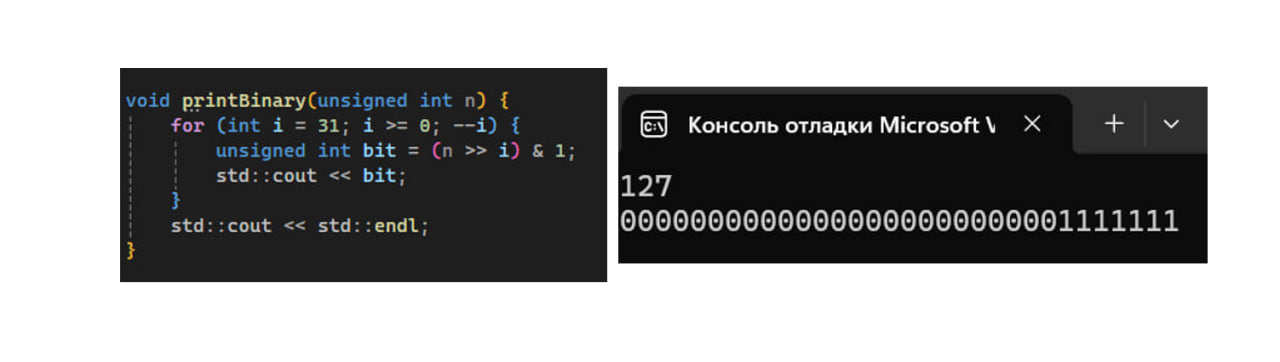
\includegraphics[width=0.99\textwidth]{0.jpg}
\end{figure} 
\section{float -> binary}
Выведем на экран вид хранения числа с плавающей точкой:
\begin{figure}[H]
    \centering
    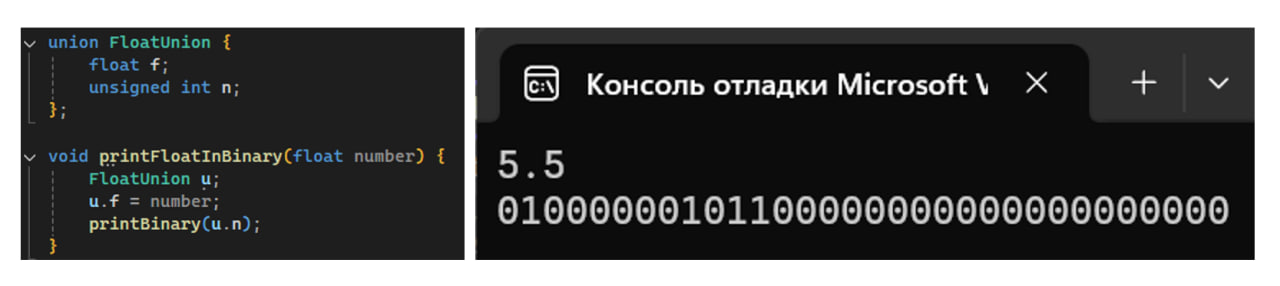
\includegraphics[width=0.99\textwidth]{1.jpg}
\end{figure} 
Расшифруем запись с экрана: Первый бит $0$ означает что число положительное. Затем идут $8$ бит экспоненты: $10000001$.\\
Затем идет мантисса $01100000000000000000000$. Таким образом число будет иметь вид $101.1$.\\
Целая часть при переводе действительно дает $5$, а дробная часть $0.5$

\section{Переполнение мантиссы}
Напишем код, который будет сохранять во float числа вида $10^n$, где n будет возрастать:

\begin{figure}[H]
    \centering
    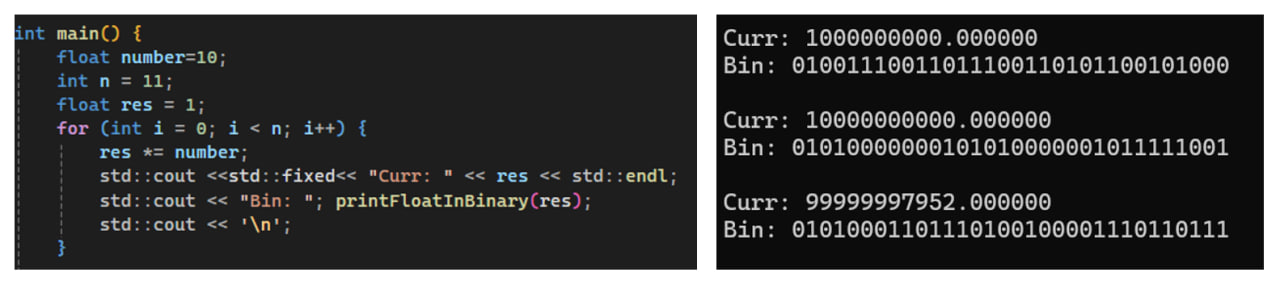
\includegraphics[width=0.99\textwidth]{2.jpg}
\end{figure} 
Запустив программу заметим, что начиная с $11$ степени, сохраненное значение вовсе не является степенью $10$:


Числа оказываются достаточно близкими к истинному значению, но чем больше степень -- тем больше разница. Это связано с дискретностью типа float.

\section{БезРиконечный Морти(цикл)}
\begin{figure}[H]
    \centering
    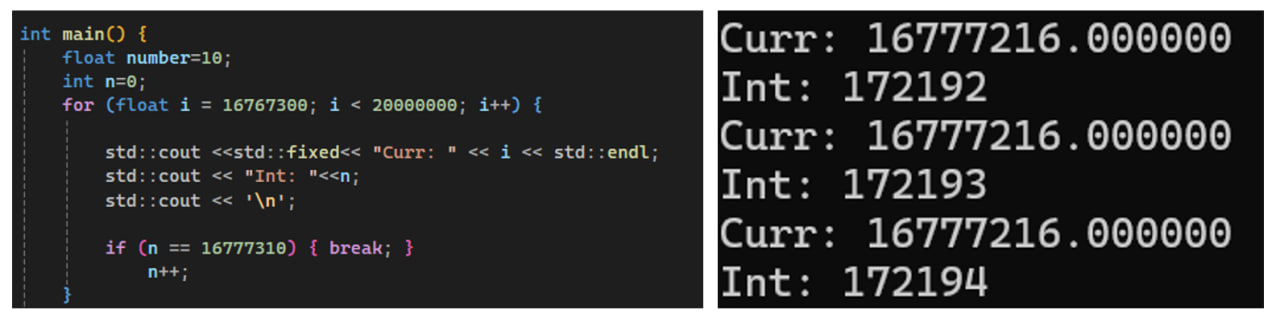
\includegraphics[width=0.99\textwidth]{3.jpg}
\end{figure} 
Выполнение кода прерывается на $16777310$, так как начиная с $16777216$ итератор цикла $i$ перестает меняться и цикл становится бесконечным:

\section{Расчет числа $\pi$(Пи)}
Будем находить число $\pi$ с помощью алгоритмов Эйлера, Лейбница, Виета и Валлиса.\\
Построим графики зависимости найденного числа от итераций для каждого алгоритма.\\
\begin{figure}[H]
    \centering
    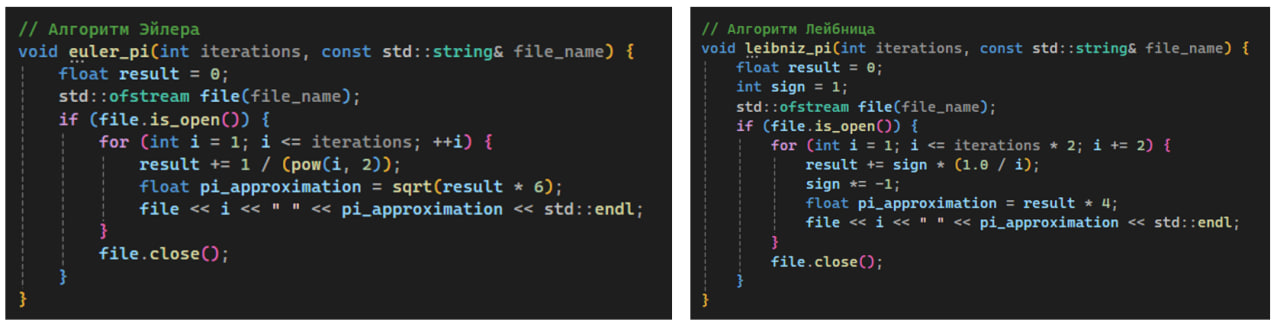
\includegraphics[width=0.99\textwidth]{4.jpg}
\end{figure} 
\begin{figure}[H]
    \centering
    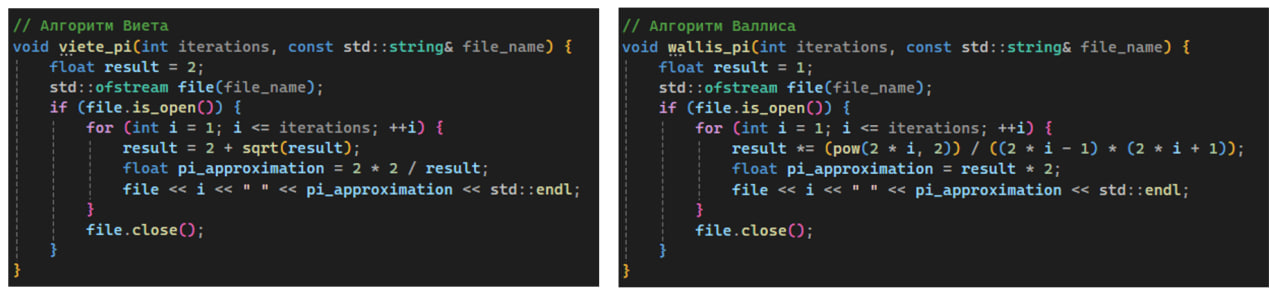
\includegraphics[width=0.99\textwidth]{5.jpg}
\end{figure} 
\subsection{Алгоритм Эйлера}

\begin{figure}[H]
    \centering
    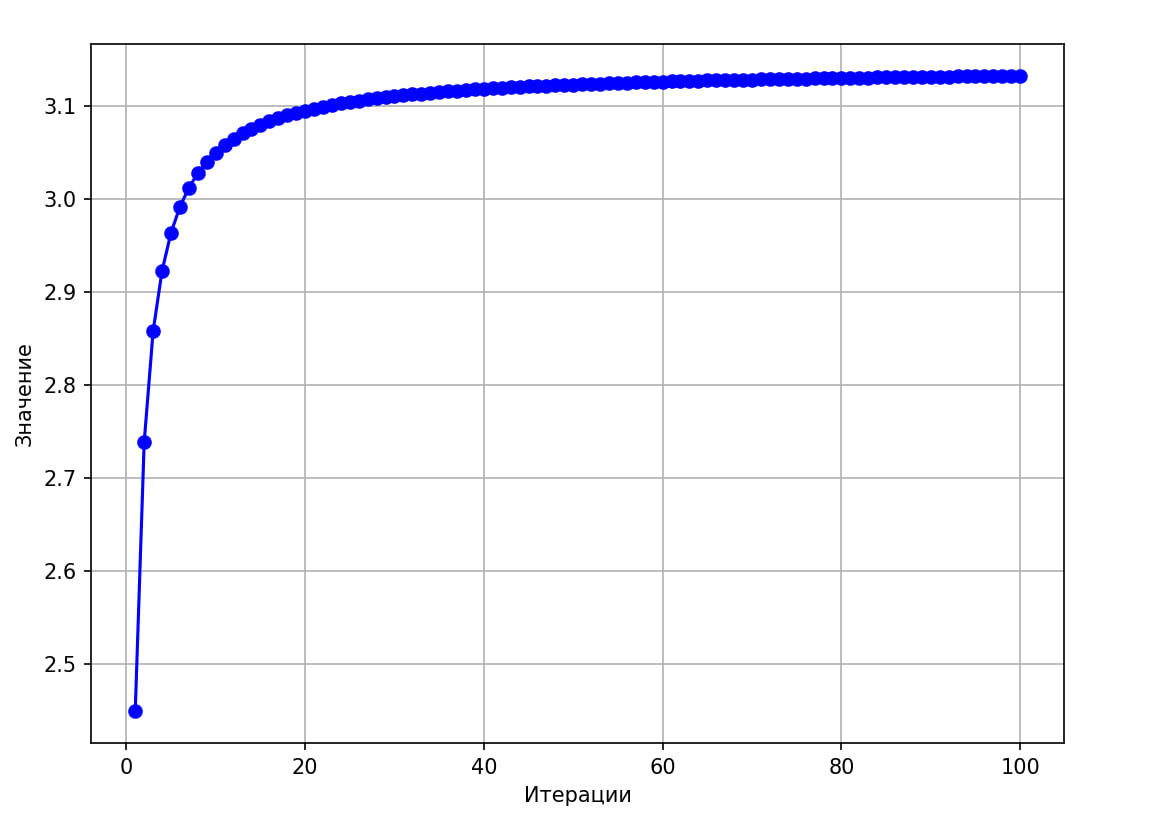
\includegraphics[width=0.7\textwidth]{6.jpg}
\end{figure} 
Алгоритм за малое количество итераций достигает значения $3.1413934230804443359375$
и больше не меняется, это связано с тем, что прибавляемые числа в алгоритме уже не могут "перескочить" до следующего значения float.

\subsection{Алгоритм Лейбница}
\begin{figure}[H]
    \centering
    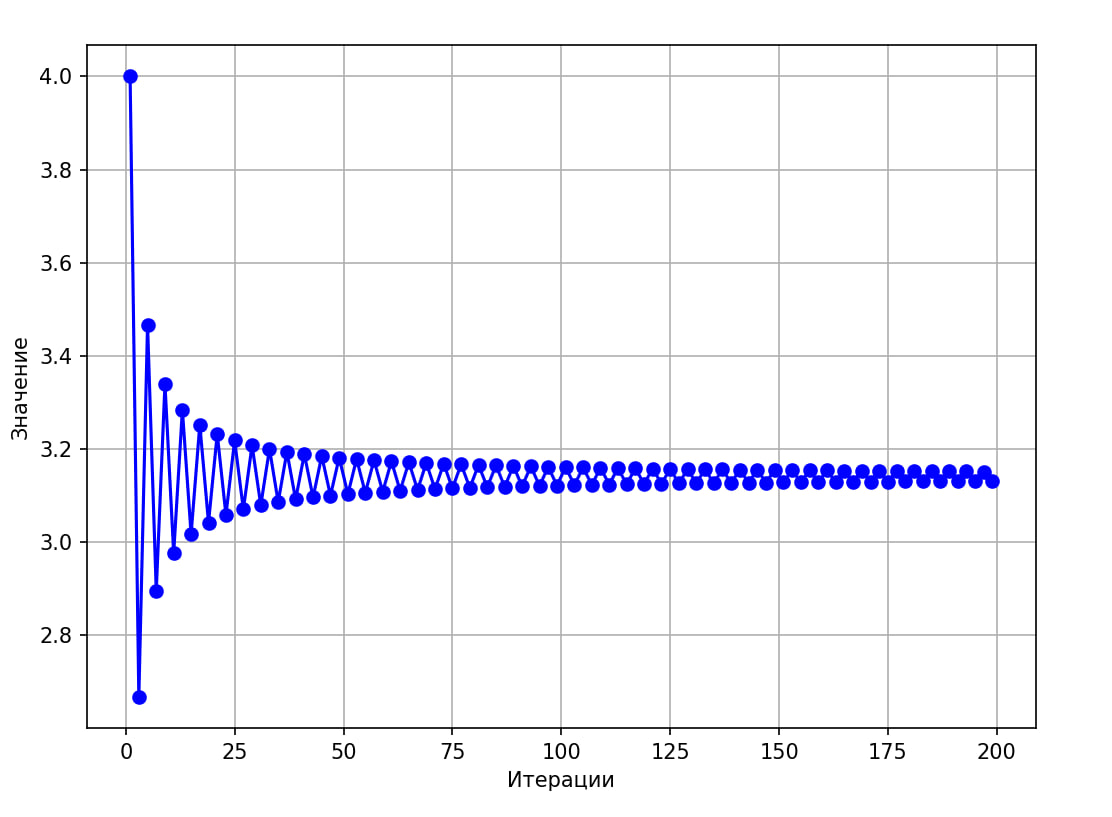
\includegraphics[width=0.7\textwidth]{7.jpg}
\end{figure} 

\subsection{Алгоритм Виета}
\begin{figure}[H]
    \centering
    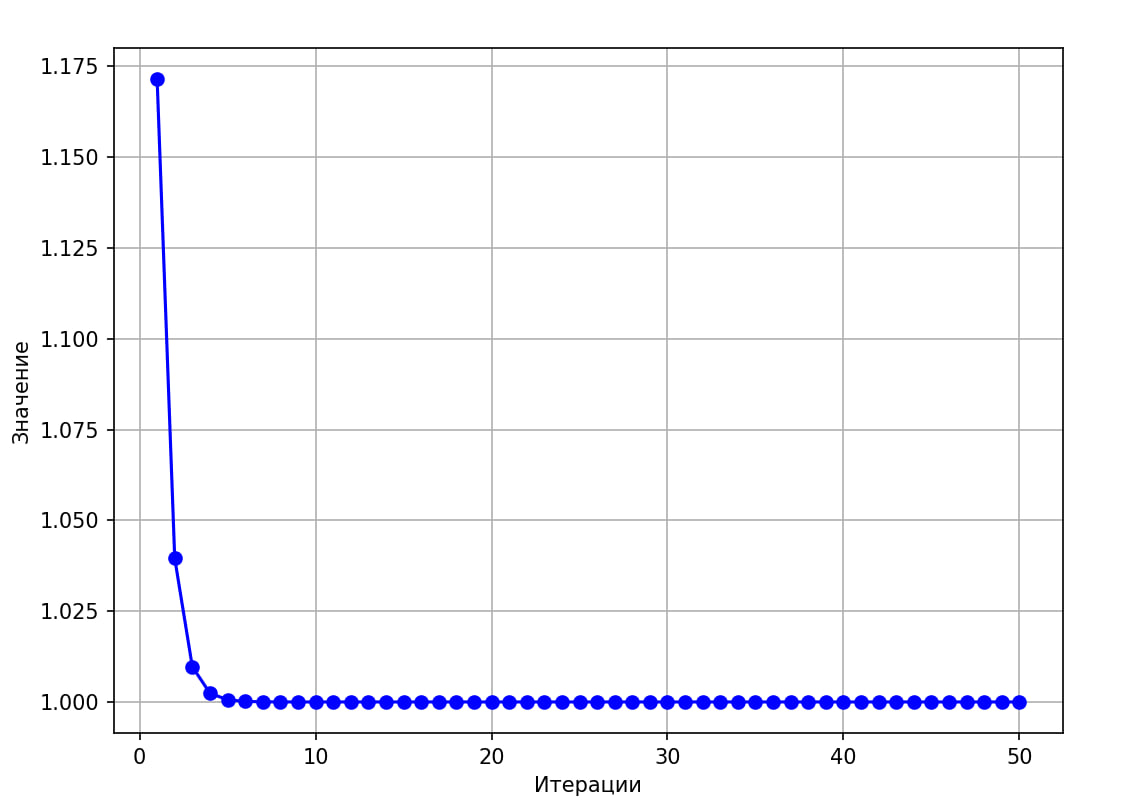
\includegraphics[width=0.7\textwidth]{8.jpg}
\end{figure} 
Этот алгоритм очень быстро ломается.

\subsection{Алгоритм Валлиса}
\begin{figure}[H]
    \centering
    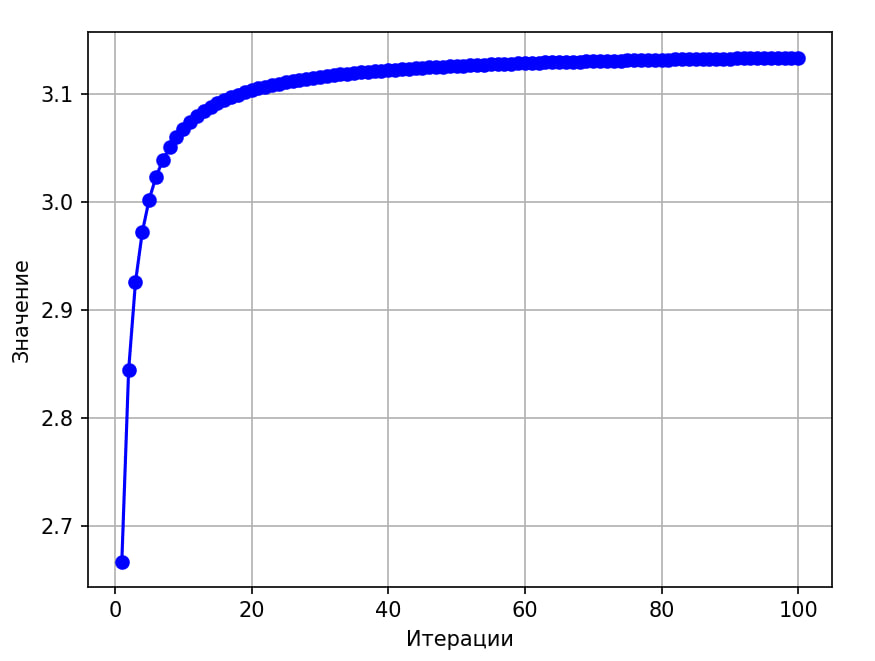
\includegraphics[width=0.7\textwidth]{9.jpg}
\end{figure} 

Алгоритм за малое количество итераций достигает значения почим истиного значения
и больше не меняется, это связано с тем, что прибавляемые числа в алгоритме уже не могут "перескочить" до следующего значения float. График напоминает алгоритм Эйлера.

\section{Время расчета числа $\pi$(Пи)}
Для каждого алгоритма выше рассчитаем то, за какое среднее время и количество итераций они достигают до каждого знака $\pi$.\\
Затем, объединим данные и построим графики:

\begin{figure}[H]
    \centering
    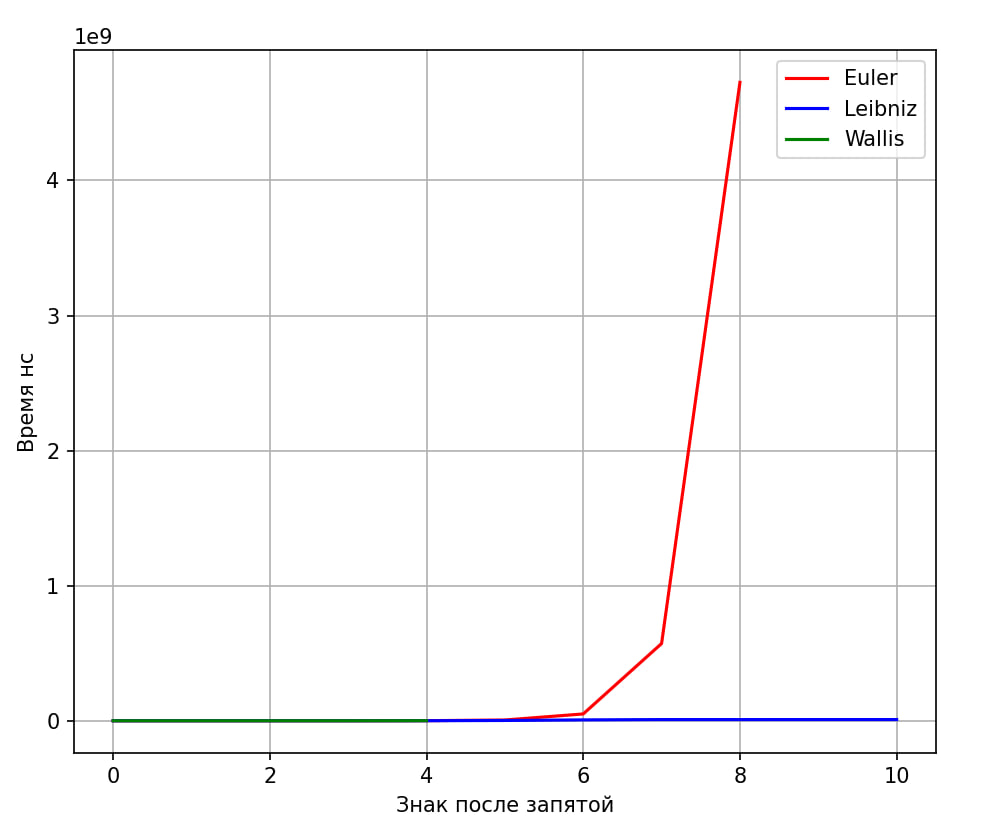
\includegraphics[width=0.6\textwidth]{10.jpg}
\end{figure} 
\begin{figure}[H]
    \centering
    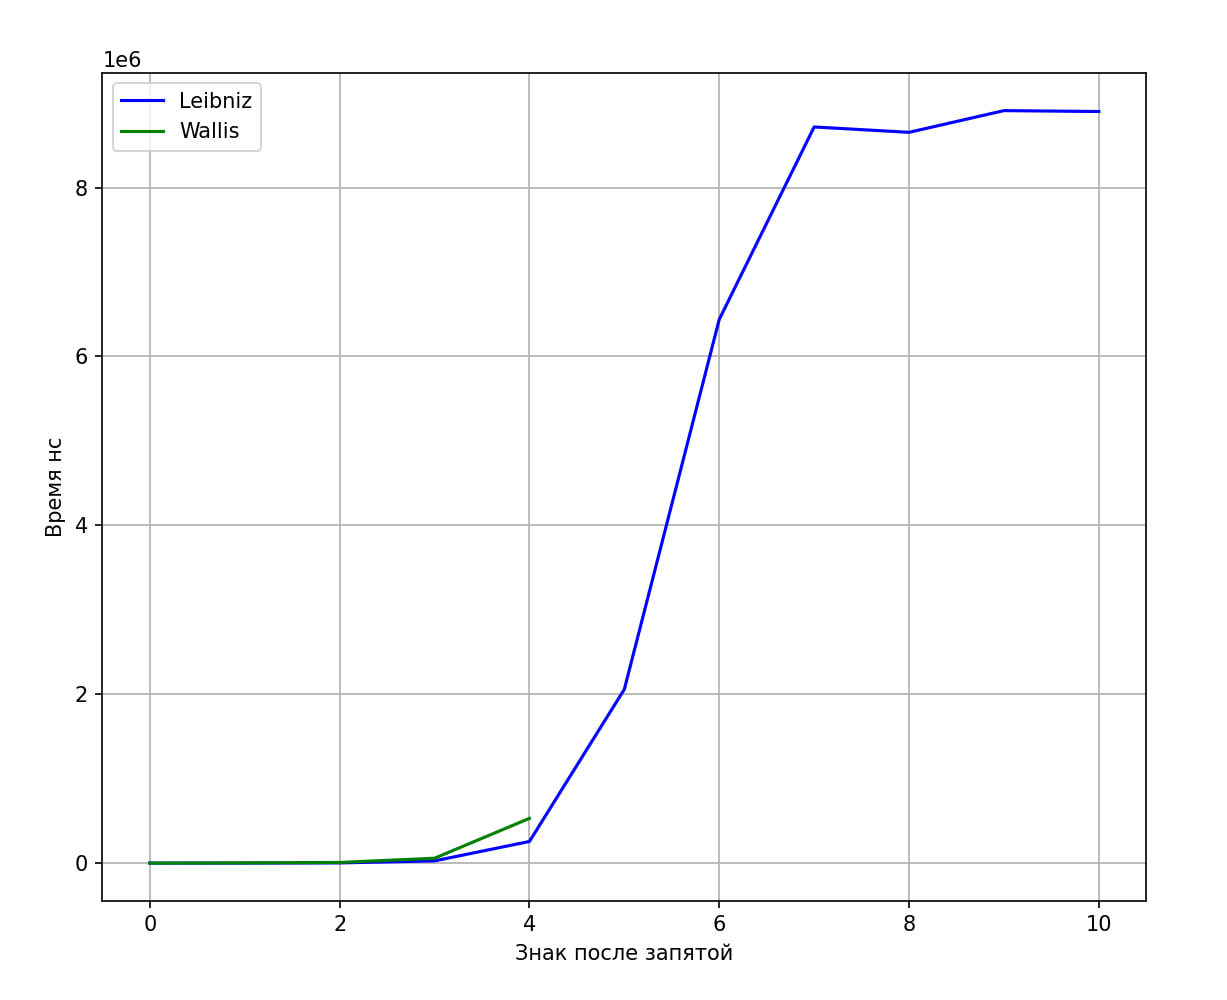
\includegraphics[width=0.7\textwidth]{11.jpg}
\end{figure} 

Алгоритм Эйлера и Валлиса оказался неспособен вычислить больше 8 знаков $\pi$ даже на типе double и поэтому его график обрывается.\\
 Самым быстрым  и точным алгоритмом оказался алгоритм Лейбница. Он также не "ломается" на больших итерациях, а просто застывает. 

\section{Вывод}
В ходе выполнения лабораторной работы было произведено определение свойств чисел с плавающей точкой, найдены ситуации с их нерпедсказуемой работой, расшифрована их записть в памяти. Произведена оценка эффективности алгоритмов поиска числа Пи на числах с плавающей точкой.
\end{document}